% 5  Conclusion
% 5.1  Discuss strengths and weaknesses within model.
% 5.2  Future improvements/future work.
% 5.3  Acknowledgements
% 5.4  Bibliography

\section{Conclusion}
	\begin{frame}
		\frametitle{Future Problems}
		Our techniques can numerically solve any model such that:
		\be
			\item $u(x,t=0) = 0$.
			\item $f(y)$ is monotone non-increasing on $y \leq 0$ and non-decreasing on $y \geq 0$.
		\ee
	\end{frame}
	
	\begin{frame}
		\frametitle{Future Problems: Non-zero initial $u$}
		What if $u(x,t=0) \neq 0$?\\
		Matt postulated that our technique would work if $u(x,t=0)$ has a similar shape to $\eta(x,t=0)$.
	\end{frame}

	\begin{frame}
		\frametitle{Future Problems: W-bumps}
		What if we have W-bumps?
		\begin{center}
			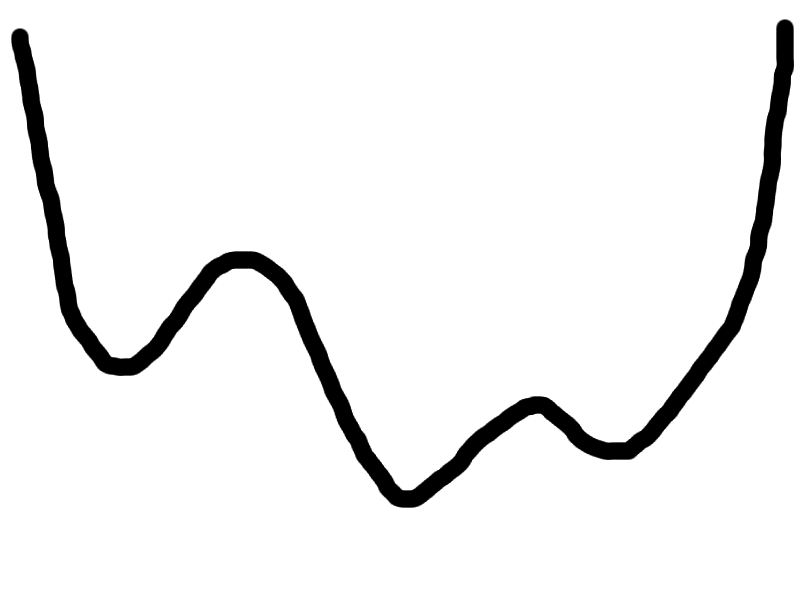
\includegraphics[width = 0.4\textwidth]{wbumps1.png}
			\quad
			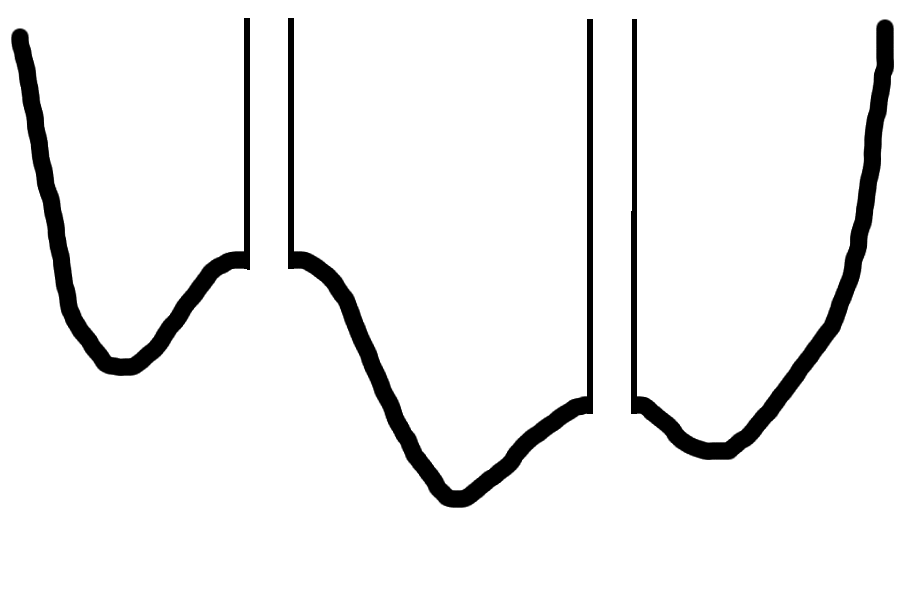
\includegraphics[width = 0.45\textwidth]{wbumps2.png}
		\end{center}
		Can we split into separate bays and analyse them separately?\\
		There are problems.
	\end{frame}


	\begin{frame}
		\frametitle{Acknowledgments}
	
		\begin{itemize}
		\item Dr. Alexei Rybkin  
		\item Dr. Dmitry Nicolsky
		\item Dr. Efim Pelinovsky
		\item Viacheslav Garayshin
		\item National Science Foundation
		\item University of Alaska Fairbanks
		\end{itemize}
		\end{frame}
	
		\begin{frame}[allowframebreaks]
		\nocite{*}
		\frametitle{Bibliography}
		\bibliographystyle{alpha}
		\bibliography{bibliography}
	\end{frame}